\documentclass[10pt]{article}

\usepackage[preprint]{tmlr}

\usepackage[utf8]{inputenc}
\usepackage{amsmath,amssymb,amsthm}
\usepackage{mathtools}
\usepackage{hyperref}
\usepackage{cleveref}
\usepackage{booktabs}
\usepackage{multirow}
\usepackage{enumitem}
\usepackage{xcolor}
\usepackage{graphicx}
\usepackage{microtype}
\usepackage{tikz}
\usetikzlibrary{arrows.meta, decorations.pathreplacing, patterns,
                shapes.geometric, positioning, calc, backgrounds, fit}
\usepackage{tcolorbox}
\tcbuselibrary{skins, breakable}

% --- colour palette ---
\definecolor{triblue}{RGB}{30,100,180}
\definecolor{trigreen}{RGB}{30,140,80}
\definecolor{trired}{RGB}{190,40,40}
\definecolor{trigold}{RGB}{200,150,0}
\definecolor{thlightblue}{RGB}{230,242,255}
\definecolor{thborderblue}{RGB}{100,160,220}
\definecolor{deflightgreen}{RGB}{236,248,236}
\definecolor{defbordergreen}{RGB}{80,160,100}
\definecolor{remlightyellow}{RGB}{255,252,230}
\definecolor{rembordergold}{RGB}{200,170,40}

% --- theorem boxes ---
\tcbset{
  thmstyle/.style={
    enhanced, breakable, sharp corners,
    boxrule=0.6pt, left=6pt, right=6pt, top=4pt, bottom=4pt,
    fonttitle=\bfseries\sffamily\small,
    attach boxed title to top left={yshift=-2mm, xshift=4mm},
    boxed title style={sharp corners, boxrule=0pt, colback=thborderblue},
    colback=thlightblue, colframe=thborderblue, coltitle=white,
  },
  defstyle/.style={
    enhanced, breakable, sharp corners,
    boxrule=0.6pt, left=6pt, right=6pt, top=4pt, bottom=4pt,
    fonttitle=\bfseries\sffamily\small,
    attach boxed title to top left={yshift=-2mm, xshift=4mm},
    boxed title style={sharp corners, boxrule=0pt, colback=defbordergreen},
    colback=deflightgreen, colframe=defbordergreen, coltitle=white,
  },
  remstyle/.style={
    enhanced, breakable, sharp corners,
    boxrule=0.5pt, left=6pt, right=6pt, top=3pt, bottom=3pt,
    colback=remlightyellow, colframe=rembordergold,
    fontupper=\small,
  },
}

\newenvironment{thmbox}[1]{%
  \begin{tcolorbox}[thmstyle, title={#1}]}{\end{tcolorbox}}
\newenvironment{defbox}[1]{%
  \begin{tcolorbox}[defstyle, title={#1}]}{\end{tcolorbox}}
\newenvironment{rembox}{%
  \begin{tcolorbox}[remstyle]}{\end{tcolorbox}}

\newtheorem{theorem}{Theorem}[section]
\newtheorem{lemma}[theorem]{Lemma}
\newtheorem{corollary}[theorem]{Corollary}
\newtheorem{proposition}[theorem]{Proposition}
\newtheorem{definition}[theorem]{Definition}
\newtheorem{remark}[theorem]{Remark}
\newtheorem{example}[theorem]{Example}

\newcommand{\R}{\mathbb{R}}
\newcommand{\B}{\mathbb{B}}
\newcommand{\N}{\mathbb{N}}
\newcommand{\dT}{\partial T}
\newcommand{\conf}{\mathrm{conf}}
\newcommand{\ans}{\mathrm{ans}}

\title{The Hallucination Trilemma: A Topological Impossibility\\
       for Faithful, Covering, and Calibrated Language Models}

\author{\name Manish Bhatt \email manish.bhatt13212@gmail.com \\
      \addr OWASP
      \AND
      \name Ken Huang \email ken@distributedapps.ai \\
      \addr Distributedapps.ai}

\def\month{05}
\def\year{2026}
\def\openreview{\url{https://openreview.net/forum?id=XXXX}}

\begin{document}

\maketitle

\begin{abstract}
We prove that no question-answering model whose confidence map is
continuous on a connected question space can simultaneously satisfy three
properties: \emph{faithful} (threshold-confidence answers are strictly
correct), \emph{covering} (the model produces both correct and incorrect
answers), and \emph{strictly calibrated} (confidence above the threshold
if and only if correct, and confidence below the threshold if and only if
incorrect). Coverage is satisfied by any model that produces both correct
and incorrect answers. The binding constraint is between faithfulness and
strict calibration: calibration turns the two coverage witnesses into
confidence values on opposite sides of the threshold; connectedness and
continuity force a threshold-confidence question; calibration pins the
truth-distance to zero there; faithfulness demands it be strictly
negative. The contradiction is structural, not statistical, but it is a
statement about this formal design target rather than a claim that current
deployed LLMs satisfy strict biconditional calibration. As calibration is
idealized toward the zero-slack biconditional form, the constraint tightens.
We call this the \textbf{Hallucination Trilemma}. The same logical core
applies without any topology when the question set contains a single
boundary example, and the formal development includes multi-turn,
stochastic, discrete, and approximate variants. The development is
machine-verified in Lean~4 against Mathlib v4.28 with no axioms beyond
the three standard Lean kernel axioms.
\end{abstract}

% ============================================================
\section{Introduction}
\label{sec:intro}

Hallucination (a model producing a confident but wrong answer) is one
of the most reliably observed problems with deployed language models
\citep{maynez2020faithfulness,ji2023survey,zhang2023siren}. Most proposed
fixes are empirical: train on more data, add RLHF, tune the temperature,
apply a post-hoc calibration method. This paper takes a different angle.
The problem is not just an engineering gap under the idealized conditions
studied here. There is a mathematical obstruction, and it does not depend
on how the model is trained.

\paragraph{The impossibility.}
Consider any model that takes a question and returns an answer together
with a confidence score. It is natural to want three things from such a
model:

\begin{itemize}[nosep,leftmargin=1.5em]
\item \textbf{Faithful:} when the model is at least half-confident, its
  answer should actually be correct.
\item \textbf{Covering:} the model should sometimes be right and sometimes
  be wrong; it should not simply refuse every question or output a
  constant answer.
\item \textbf{Calibrated:} confidence should track correctness in both
  directions. High confidence should mean the answer is right; low
  confidence should mean it is wrong.
\end{itemize}

For a continuous confidence map on a connected question space, these three
properties cannot coexist. The proof requires no training assumptions, no
architecture details, no statistics. It is an application of the intermediate
value theorem.

\paragraph{Why.}
If the model is covering, there is a question $q_+$ where its answer is
correct and a question $q_-$ where its answer is wrong. Calibration converts
these into statements about the confidence score: above $\tfrac{1}{2}$ at
$q_+$ and below $\tfrac{1}{2}$ at $q_-$.
If the question space is connected and the confidence map is continuous,
the intermediate value theorem forces the confidence to hit $\tfrac{1}{2}$
at some question, call it $q_0$. Calibration then forces the model's answer
at $q_0$ to sit on the truth boundary. But
faithfulness says: if you are at least half-confident, you must be
strictly correct. At $q_0$ the model is exactly half-confident, which is
enough for faithfulness to fire, and the answer is on the boundary, which
is not strictly correct. Contradiction.

\paragraph{What the result says about real models.}
Coverage is satisfied by any model that produces both correct and incorrect answers: every useful LLM
produces both correct and incorrect answers. The binding question is
calibration. The theorem does not say that current deployed LLMs satisfy
all three conditions and derive a contradiction; no current model
satisfies strict biconditional calibration. What it says is that the
formal design target (a model that is simultaneously faithful, strictly
calibrated, covering, and continuous in the confidence coordinate on a
connected question space) is unreachable. As a model is idealized toward
zero-slack calibration, the constraint between calibration and faithfulness
tightens. \Cref{sec:approx} makes this precise: under
$\varepsilon$-calibration and $\varepsilon$-coverage, a threshold-confidence
question has truth-distance in $[-\varepsilon,0)$. At zero slack this becomes
the exact contradiction $0 \leq \delta_M(q_0) < 0$.
The obstruction is structural, not a matter of insufficient training.

\paragraph{What distinguishes this from prior work.}
\citet{xu2024hallucination} prove hallucination via computability: a finite
model cannot represent all computable functions, so out-of-distribution
inputs will always find gaps. That argument concerns model capacity at the
distribution boundary and says nothing about calibration.
\citet{karpowicz2025impossibility} prove a conflict among four conditions
(truthful response generation, semantic information conservation, relevant
knowledge revelation, knowledge-constrained optimality) via mechanism design
and proper scoring rules. Neither proof uses the IVT; neither makes
calibration a central condition.

The present result is distinguished by three things: the conditions are
different (three, with calibration explicit), the proof uses only IVT and
connectedness, and it is machine-verified. It is, to our knowledge, the
first hallucination impossibility formalized in a proof assistant.

\paragraph{Contributions.}
\begin{itemize}[nosep,leftmargin=1.5em]
\item \textbf{The Hallucination Trilemma} (Theorems
  \ref{thm:boundary}--\ref{thm:trilemma}): faithful, covering, and
  calibrated are mutually inconsistent for any continuous model on a
  connected question space. Each of the three conditions is individually
  necessary.
\item \textbf{Discrete core} (Theorem \ref{thm:pure-discrete}): on any
  set with no topology at all, a single boundary question suffices to
  derive the same contradiction. The continuous result factors through
  this two-line logical core; IVT is used only to produce the boundary
  question, not to deliver the contradiction.
\item \textbf{Extensions}: multi-turn conversations (Theorem
  \ref{thm:multi-turn}), stochastic models with a positive-probability
  hallucination guarantee (Theorem \ref{thm:dichotomy}), and an antipodal
  variant where coverage follows from the structure of the question space.
\item \textbf{Approximate bridge} (\Cref{sec:approx}): under
  $\varepsilon$-calibration, the impossibility becomes quantitative.
  A threshold-confidence question $q_0$ exists with
  $\delta_M(q_0) \in [-\varepsilon, 0)$; improving calibration tightens this
  margin. This connects the idealized result to approximate real models and
  localises the failure to the
  in-distribution/OOD transition band (Corollary \ref{cor:ood}).
\item \textbf{Lean formalization}: all results are machine-verified in
  Lean 4 against Mathlib v4.28, no \texttt{sorry}, headline theorems
  dependent only on the three standard Lean kernel axioms.
\end{itemize}

% ============================================================
\section{Setup}
\label{sec:setup}

We work with a minimal abstract model of a question-answering system. The
formalism is general enough to cover any model that returns an answer
alongside a confidence score, whether that score comes from a softmax
probability, a calibrated estimator, or a learned scalar head.

\paragraph{The model.}
Let $Q$ be the \emph{question space}, a connected topological space,
and $A$ the \emph{answer space}. A \emph{model} is a continuous map
$M\colon Q \to A \times \R$. The two components are:
\[
  \ans(q) = (M(q))_1 \;\in A, \qquad \conf(q) = (M(q))_2 \;\in \R.
\]
Connectedness of $Q$ is the key topological assumption; it says the
question space is not split into separated pieces. The Lean proof uses
connectedness (more precisely, preconnectedness of the whole space) and
continuity of the confidence coordinate; it does not require a path between
every two questions. Path-connected embedding spaces are important examples,
but the theorem is stated at the weaker connectedness level. When $Q$ is
genuinely discrete, two-sided coverage alone does not force a threshold
crossing; the discrete result of \Cref{sec:discrete} applies instead when a
boundary question is present.

\paragraph{Measuring correctness.}
Rather than a binary right/wrong label, we use a continuous
\emph{truth-distance} $\delta\colon Q \times A \to \R$. The sign encodes
correctness: $\delta(q,a) < 0$ means the answer $a$ is correct at
question $q$, $\delta(q,a) > 0$ means it is wrong, and $\delta(q,a) = 0$
is the boundary between the two. We write $\delta_M(q)$ for the
truth-distance of the model's own answer: $\delta_M(q) = \delta(q, \ans(q))$.

This signed-distance formulation is general. It covers continuous
relaxations of binary correctness, soft factuality scores, semantic
similarity thresholds, and other scoring functions with a natural zero.
A discontinuous two-valued label $\delta=\pm1$ on a connected domain cannot
itself satisfy both continuity and two-sided coverage; in that case the
discrete theorem, or a continuous surrogate score, is the relevant formal
object.

\paragraph{The threshold $\tfrac{1}{2}$.}
The conditions use $\tfrac{1}{2}$ as the boundary between high and low
confidence. This is conventional: it is the natural 50/50 point where
the model considers itself equally likely to be right or wrong, but not
mathematically necessary. Replacing $\tfrac{1}{2}$ with any constant
$c \in \R$ throughout gives an equivalent theorem with an identical proof:
coverage produces witnesses above and below $c$, connectedness forces a
crossing at $c$, calibration pins $\delta_M = 0$ there, faithfulness
demands $\delta_M < 0$ there. The impossibility holds at whatever
threshold the three conditions share.

\paragraph{Why these three conditions.}
The three conditions are the tightest set that creates the impossibility:
each pair of two is simultaneously achievable (\Cref{sec:counterexamples});
all three together are not (\Cref{thm:trilemma}).

Coverage is a weak condition. It requires only that the model produce at
least one correct answer and at least one wrong answer across its question
domain. It is the hypothesis that gives the IVT argument its two witnesses
$q_+$ and $q_-$; without it, the confidence map need not cross the threshold
at all. In the proof it is load-bearing even though in practice any
model that produces both correct and incorrect answers satisfies it.

\paragraph{The three conditions.}
We now define the three properties precisely.

\begin{definition}[Faithfulness]
\label{def:faithful}
$M$ is \emph{faithful} if, for every question $q$:
\[
  \conf(q) \geq \tfrac{1}{2} \;\Longrightarrow\; \delta_M(q) < 0.
\]
When the model is at least half-confident, its answer is strictly correct.
\end{definition}

\begin{definition}[Coverage]
\label{def:covering}
$M$ satisfies \emph{coverage} if there exist questions $q_+, q_- \in Q$
with $\delta_M(q_+) < 0$ (a correct answer) and $\delta_M(q_-) > 0$
(a wrong answer). The model is not trivially correct everywhere or
trivially wrong everywhere.
\end{definition}

\begin{definition}[Strict calibration]
\label{def:calibrated}
$M$ is \emph{strictly calibrated} if, for every question $q$:
\[
  \conf(q) > \tfrac{1}{2} \;\iff\; \delta_M(q) < 0
  \qquad\text{and}\qquad
  \conf(q) < \tfrac{1}{2} \;\iff\; \delta_M(q) > 0.
\]
Confidence above $\tfrac{1}{2}$ is exactly equivalent to being correct;
confidence below $\tfrac{1}{2}$ is exactly equivalent to being wrong.
\end{definition}

Strict calibration is a biconditional between the sign of the confidence
relative to the threshold and the sign of the truth-distance. It is different
from the usual statistical notion of calibration (where $\conf(q)$ approximates
the probability of correctness), and is best read as an idealized threshold
calibration condition. It is the condition that gives the IVT argument its
bite: it pins the truth-distance to zero wherever the confidence crosses
$\tfrac{1}{2}$.

% ============================================================
\section{The Hallucination Trilemma}
\label{sec:trilemma}

The argument has two steps. First we show that coverage and calibration
together force a ``boundary question'': a question where the
model sits exactly halfway between confident and uncertain, and whose
answer lands exactly on the truth boundary. Then faithfulness fires at
that question and produces a contradiction.

\begin{theorem}[Boundary question]
\label{thm:boundary}
Let $Q$ be connected and $M$ be a continuous model with continuous
truth-distance $\delta$. If $M$ is covering and strictly calibrated, then
there is a question $q_0 \in Q$ where $\conf(q_0) = \tfrac{1}{2}$ and
$\delta_M(q_0) = 0$.
\end{theorem}

\begin{proof}
Coverage gives $q_+$ with $\delta_M(q_+) < 0$ and $q_-$ with $\delta_M(q_-)
> 0$. Applying strict calibration at each witness: $\conf(q_+) > \tfrac{1}{2}$
and $\conf(q_-) < \tfrac{1}{2}$.

The confidence map $q \mapsto \conf(q)$ is continuous on the connected
space $Q$. By the intermediate value theorem, it must take the value
$\tfrac{1}{2}$ somewhere; call that question $q_0$.

At $q_0$ the confidence is exactly $\tfrac{1}{2}$, so it is neither above
nor below. The two biconditionals of strict calibration then both fire in
the negative direction: $\delta_M(q_0)$ is not $< 0$ (from the first
biconditional) and not $> 0$ (from the second). Therefore $\delta_M(q_0)
= 0$.
\end{proof}

\begin{theorem}[Hallucination Trilemma]
\label{thm:trilemma}
No continuous model on a connected question space is simultaneously
faithful, covering, and strictly calibrated.
\end{theorem}

\begin{proof}
By \Cref{thm:boundary}, there is a question $q_0$ with $\conf(q_0) =
\tfrac{1}{2}$ and $\delta_M(q_0) = 0$. Since $\conf(q_0) = \tfrac{1}{2}
\geq \tfrac{1}{2}$, faithfulness requires $\delta_M(q_0) < 0$. But
$\delta_M(q_0) = 0$. Contradiction.
\end{proof}

The proof uses no facts about the model's architecture, training
procedure, or parameter count. It uses only the continuity of $M$ and
the connectedness of $Q$. Any model (transformer, MLP, nearest-neighbor,
or retrieval-augmented) that satisfies the three conditions would have to
violate one of these two properties.

\paragraph{Tightness.}
\label{par:tightness}
The impossibility is tight: relaxing the faithfulness threshold by any
$\varepsilon > 0$ breaks it. The model $Q = [0,1]$, $\conf(q) = 1-q$,
$\delta_M(q) = q - \tfrac{1}{2}$ satisfies strict calibration and
coverage. It satisfies $(\tfrac{1}{2}+\varepsilon)$-faithfulness
($\conf \geq \tfrac{1}{2}+\varepsilon \Rightarrow q \leq
\tfrac{1}{2}-\varepsilon \Rightarrow \delta_M \leq -\varepsilon < 0$)
for every $\varepsilon > 0$, but fails standard faithfulness at $q =
\tfrac{1}{2}$ where $\conf = \tfrac{1}{2}$ and $\delta_M = 0$.
A model satisfying $(\tfrac{1}{2}+\varepsilon)$-faithfulness provides no
faithfulness guarantee for questions with confidence in
$[\tfrac{1}{2},\tfrac{1}{2}+\varepsilon)$; that threshold band is the price
of escaping while preserving strict calibration and coverage.

\begin{figure}[t]
\centering
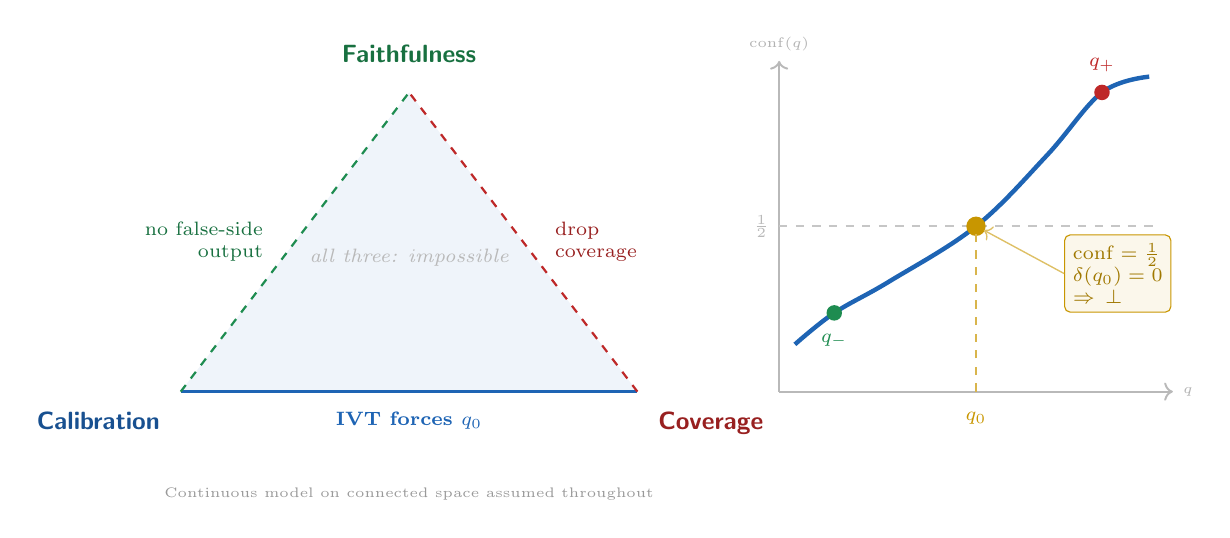
\begin{tikzpicture}[x=1cm, y=1cm]

%% ════════════════════════════════════════════════════════════════
%% LEFT PANEL – the trilemma triangle  (fits in 0..6.2 x -1.8..5.0)
%% ════════════════════════════════════════════════════════════════

% triangle vertices (inside, away from labels)
\coordinate (TF) at (3.1, 3.8);   % Faithfulness – top
\coordinate (TC) at (0.2, 0);     % Calibration  – bottom-left
\coordinate (TV) at (6.0, 0);     % Coverage     – bottom-right

% shaded interior
\fill[triblue!7] (TF) -- (TC) -- (TV) -- cycle;

% edges
\draw[triblue,  very thick]              (TC) -- (TV); % bottom: main result
\draw[trigreen, thick, dashed]           (TC) -- (TF); % left
\draw[trired,   thick, dashed]           (TV) -- (TF); % right

% ── vertex labels well outside the corners ──
\node[above, font=\small\bfseries\sffamily, text=trigreen!80!black]
  at (3.1, 4.05) {Faithfulness};

\node[below left, font=\small\bfseries\sffamily, text=triblue!80!black,
      xshift=-4pt, yshift=-4pt]
  at (TC) {Calibration};

\node[below right, font=\small\bfseries\sffamily, text=trired!80!black,
      xshift=4pt, yshift=-4pt]
  at (TV) {Coverage};

% ── edge midpoints (used for annotations) ──
% bottom edge midpoint: (3.1, 0)
\node[below, yshift=-4pt, font=\scriptsize, text=triblue, align=center]
  at (3.1, 0) {\textbf{IVT forces $q_0$}};

% left edge midpoint: ((0.2+3.1)/2, (0+3.8)/2) = (1.65, 1.9)
% annotation placed to the left of the midpoint
\node[left, xshift=-8pt, font=\scriptsize, text=trigreen!80!black, align=right]
  at (1.65, 1.9) {no false-side\\output};

% right edge midpoint: ((6.0+3.1)/2, (0+3.8)/2) = (4.55, 1.9)
% annotation placed to the right of the midpoint
\node[right, xshift=8pt, font=\scriptsize, text=trired!80!black, align=left]
  at (4.55, 1.9) {drop\\coverage};

% centre label
\node[font=\scriptsize\itshape, text=gray!55]
  at (3.1, 1.7) {all three: impossible};

% footnote below whole triangle
\node[font=\tiny, text=black!40, align=center]
  at (3.1, -1.3) {Continuous model on connected space assumed throughout};

%% ════════════════════════════════════════════════════════════════
%% RIGHT PANEL – the IVT crossing  (shift by 7.8 in x)
%% ════════════════════════════════════════════════════════════════
\begin{scope}[shift={(7.8, 0)}]

  % axes
  \draw[->, gray!55, line width=0.7pt] (0, 0) -- (5.0, 0)
    node[right, font=\tiny, text=gray!60] {$q$};
  \draw[->, gray!55, line width=0.7pt] (0, 0) -- (0, 4.2)
    node[above, font=\tiny, text=gray!60] {$\mathrm{conf}(q)$};

  % threshold line at y=2.1 (= 1/2 of 4.2)
  \draw[gray!45, dashed, line width=0.6pt] (0, 2.1) -- (4.8, 2.1);
  \node[left, font=\tiny, text=gray!55] at (0, 2.1) {$\tfrac{1}{2}$};

  % sigmoid curve through three named points:
  %   q- at x=0.7, conf≈0.45   →  y=0.45*4.2 ≈ 1.0   (below 1/2)
  %   q0 at x=2.5, conf=0.50   →  y=2.1               (exactly 1/2)
  %   q+ at x=4.1, conf≈0.90   →  y=3.8               (above 1/2)
  \draw[triblue, line width=1.6pt] plot[smooth, tension=0.6] coordinates
    {(0.2,0.6) (0.7,1.0) (1.4,1.4) (2.5,2.1) (3.4,3.0) (4.1,3.8) (4.7,4.0)};

  % q- dot and label  (below the curve, no overlap)
  \fill[trigreen] (0.7, 1.0) circle (2.8pt);
  \node[below, yshift=-4pt, font=\scriptsize, text=trigreen] at (0.7, 1.0)
    {$q_-$};

  % q+ dot and label  (above the curve, no overlap)
  \fill[trired] (4.1, 3.8) circle (2.8pt);
  \node[above, yshift=4pt, font=\scriptsize, text=trired] at (4.1, 3.8)
    {$q_+$};

  % q0 dot, vertical drop, label below x-axis
  \fill[trigold] (2.5, 2.1) circle (3.5pt);
  \draw[trigold!70, dashed, line width=0.7pt] (2.5, 0) -- (2.5, 2.1);
  \node[below, yshift=-4pt, font=\scriptsize\bfseries, text=trigold]
    at (2.5, 0) {$q_0$};

  % callout box for q0 – placed well to the right with a leader line
  \node[draw=trigold, fill=trigold!8, rounded corners=2pt,
        font=\scriptsize, text=trigold!80!black, align=left,
        inner sep=3pt] (callout)
    at (4.3, 1.5) {$\mathrm{conf}=\tfrac{1}{2}$\\$\delta(q_0)=0$\\$\Rightarrow\,\bot$};
  \draw[->, trigold!60, line width=0.5pt] (callout.west) -- (2.6, 2.05);

\end{scope}

\end{tikzpicture}
\vspace{2pt}
\caption{\textbf{Left:} The Hallucination Trilemma. For any continuous model on a connected space,
no model satisfies all three. The blue (solid) edge is the main result;
dashed edges correspond to counterexamples (\S\ref{sec:counterexamples}).
\textbf{Right:} The IVT argument.
Coverage gives $q_-$ (confidence $<\tfrac{1}{2}$) and $q_+$ (confidence
$>\tfrac{1}{2}$); connectedness forces the crossing $q_0$; calibration
pins $\delta(q_0)=0$; faithfulness then demands $\delta(q_0)<0$ --
contradiction.}
\label{fig:trilemma}
\end{figure}

\subsection{Each hypothesis is necessary}
\label{sec:counterexamples}

Figure~\ref{fig:trilemma} (left) presents the trilemma with three vertices:
Faithfulness, Calibration, and Coverage, all under the assumption
of a continuous model on a connected space. Each of the three is individually necessary: the
three counterexamples below show that dropping any one allows the other
two to be satisfied. Separately, the exact faithfulness threshold is
load-bearing: \S\ref{par:tightness} shows that raising the threshold by any
$\varepsilon > 0$ allows strict calibration and coverage to coexist with the
weakened faithfulness condition.

\smallskip
\noindent\textit{Covering + Calibrated + Continuous, not Faithful.}
Take $Q = [0,1]$, $\conf(q) = 1 - q$, $\delta_M(q) = q - \tfrac{1}{2}$.
Strict calibration holds: $\conf > \tfrac{1}{2} \iff q < \tfrac{1}{2}
\iff \delta_M < 0$, and $\conf < \tfrac{1}{2} \iff \delta_M > 0$.
Coverage holds: $q = \tfrac{1}{4}$ gives $\delta_M < 0$; $q = \tfrac{3}{4}$
gives $\delta_M > 0$. Faithfulness fails at $q = \tfrac{1}{2}$: $\conf =
\tfrac{1}{2} \geq \tfrac{1}{2}$ but $\delta_M = 0$, not $< 0$.
(This is the same model used for the tightness argument in
\S\ref{par:tightness}.)

\smallskip
\noindent\textit{Faithful + Calibrated + Continuous, not Covering.}
Take any model with constant $\conf = \tfrac{3}{4}$ and $\delta_M(q) < 0$
everywhere. Faithfulness: $\tfrac{3}{4} \geq \tfrac{1}{2} \Rightarrow \delta_M
< 0$. Calibration: $\conf > \tfrac{1}{2}$ and $\delta_M < 0$ are both always
true, so the first biconditional holds; the second ($\conf < \tfrac{1}{2}
\iff \delta_M > 0$) holds vacuously since both sides are always false.
Coverage fails: no wrong-answer witness $q_-$ exists.

\smallskip
\noindent\textit{Faithful + Covering + Calibrated, not Continuous.}
On $Q = [0,1]$ with $Q^+ = (\tfrac{1}{2},1]$ and $Q^- = [0,\tfrac{1}{2})$,
set $\conf(q) = \tfrac{3}{4}$ on $Q^+$ and $\conf(q) = \tfrac{1}{4}$ on
$Q^-$, with $\delta_M < 0$ on $Q^+$ and $\delta_M > 0$ on $Q^-$.
Faithfulness, coverage, and strict calibration all hold pointwise. However,
the confidence map has a jump discontinuity at $q = \tfrac{1}{2}$ and so
does not satisfy the theorem's continuity hypothesis. The model is not
continuous, not the three conditions failing; continuity is what the
impossibility requires.

% ============================================================
\section{Extensions}
\label{sec:extensions}

Three natural objections to the core result suggest possible escapes.
This section closes all three.

\begin{center}
\small
\renewcommand{\arraystretch}{1.3}
\begin{tabular}{lll}
\toprule
\textbf{Objection} & \textbf{Proposed escape} & \textbf{Result} \\
\midrule
Single-turn only & History-dependent $M: Q^T \to A\times\R$ & $Q^T$ connected; trilemma applies \\
Deterministic & Stochastic model & Dichotomy: wrong answers w.p.\ $>0$ \\
\multirow{2}{*}{Connected space} & Discrete, no boundary $q^*$ & Genuine escape (all three hold) \\
 & Discrete, with boundary $q^*$ & Same contradiction; no topology needed \\
\bottomrule
\end{tabular}
\end{center}

\subsection{Multi-turn conversations}
\label{sec:multi-turn}

\textit{Objection:} A model that sees prior conversation turns can use
context to avoid the boundary question by identifying that $q_0$ is
dangerous and respond differently based on history.

\textit{Why it fails:} The history space $Q^T$ is connected whenever $Q$
is connected, since a finite product of connected spaces is connected. The
trilemma applies to $M\colon Q^T \to A \times \R$ without modification.
The boundary question now exists in history space rather than single-turn
space, but it cannot be avoided. Context is not the issue; topology is.

\begin{theorem}[Multi-turn trilemma]
\label{thm:multi-turn}
If $Q$ is connected, any continuous, faithful, covering, and calibrated
history-dependent model $M\colon Q^T \to A \times \R$ does not exist.
\end{theorem}

\begin{proof}
$Q^T$ is connected. Apply \Cref{thm:trilemma}.
\end{proof}

A secondary observation: any $t$-turn history space can be injectively embedded
into a $t'$-turn history space (for $t' > t$) by padding with a fixed
question (\texttt{HoF\_11.adversary\_boundary\_reachable}). This is a
structural embedding of history spaces; whether a particular model preserves
the trilemma hypotheses after padding is a model-specific question.

\subsection{Probabilistic models}
\label{sec:stochastic}

\textit{Objection:} A randomized model can spread probability mass across
multiple answers at the boundary question, avoiding any single committed
wrong output.

\textit{Why it fails:} Randomization does not remove the boundary question.
The expected-value trilemma applies to the expected maps and yields a $q_0$
with $\mathbb{E}[\delta_M(q_0)] = 0$. The stochastic dichotomy
(\Cref{thm:dichotomy}) then shows that any model answering with positive
probability at or above the confidence threshold at $q_0$ must produce
wrong answers there with positive
probability.

A stochastic model draws an answer-confidence pair $(a, c)$ from a
distribution $M(q)$ rather than returning a single value. There are two
ways to extend the trilemma to this setting.

The first is immediate. Let $\bar{c}(q) = \mathbb{E}_{M(q)}[c]$ and
$\bar{\delta}(q) = \mathbb{E}_{M(q)}[\delta(q,\cdot)]$ be the expected
confidence and expected truth-distance. Assume both maps are continuous
from $Q$ to $\R$ (this requires the distribution $M(q)$ to vary
continuously with $q$ in an appropriate sense, e.g., weakly). If
$(\bar{c}, \bar{\delta})$ satisfy the three conditions in expectation,
the trilemma applies directly via \Cref{thm:trilemma}, yielding $q_0$
with $\bar{c}(q_0) = \tfrac{1}{2}$ and $\bar{\delta}(q_0) = 0$.

The second result is sharper. It weakens faithfulness from expectations
to individual samples, and shows that randomization at $q_0$ cannot help.

\begin{theorem}[Stochastic dichotomy]
\label{thm:dichotomy}
Let $(\Omega, \mu)$ be a probability space and $c, d\colon \Omega \to \R$
measurable functions with $d$ integrable. Suppose $\int d\,d\mu = 0$,
individual-sample faithfulness holds
$\mu$-almost everywhere ($c(\omega) \geq \tfrac{1}{2} \Rightarrow d(\omega)
< 0$), and $\mu\{c \geq \tfrac{1}{2}\} > 0$. Then $\mu\{d > 0\} > 0$.
\end{theorem}

\begin{proof}
Suppose $\mu\{d > 0\} = 0$, so $d \leq 0$ $\mu$-a.e.\ Then $-d \geq 0$
a.e.\ and $\int(-d)\,d\mu = 0$. A non-negative integrable function with zero
integral equals zero almost everywhere
(\texttt{integral\_eq\_zero\_iff\_of\_nonneg\_ae}), so $d = 0$ $\mu$-a.e.
But on the positive-probability set $\{c \geq \tfrac{1}{2}\}$, sample
faithfulness gives $d < 0$ a.e. A positive-probability set cannot
simultaneously satisfy $d < 0$ a.e.\ and $d = 0$ a.e. Contradiction.
\end{proof}

A stochastic model at $q_0$ with positive-probability high-confidence
outputs must produce wrong answers at $q_0$ with positive probability.
Figure~\ref{fig:extensions}(a) shows the dichotomy geometrically.

\begin{figure}[t]
\centering
\tikzset{
  fbox/.style={draw=#1, fill=#1!9, rounded corners=3pt,
               font=\scriptsize\sffamily, align=center,
               inner sep=5pt, minimum width=2.6cm, minimum height=0.75cm},
  farr/.style={-{Stealth[length=5pt,width=4pt]}, line width=1pt, #1},
}
\begin{tikzpicture}[x=1cm, y=1cm]

%% ════════════════════════════════════════════════════════════════
%% LEFT PANEL – stochastic dichotomy   (0..5.5 x -0.6..4.5)
%% ════════════════════════════════════════════════════════════════

% panel title above
\node[font=\small\bfseries\sffamily, anchor=north] at (2.75, 4.5)
  {(a) Stochastic dichotomy at $q_0$};

% x-axis
\draw[->, gray!50, line width=0.7pt] (-0.2, 0) -- (5.3, 0)
  node[right, font=\tiny, text=gray!55] {$\delta$};

% dividing line at delta = 0, placed at x=2.65
\draw[gray!40, dashed, line width=0.7pt] (2.65, -0.4) -- (2.65, 3.6);
\node[below, font=\tiny, text=gray!50] at (2.65, -0.4) {$0$};

% LEFT region label (above blue area)
\node[font=\scriptsize, text=triblue!80!black, align=center]
  at (1.35, 3.8) {\textit{boundary determinism}\\[1pt]$\delta\leq 0$ a.s.};

% RIGHT region label (above red area)
\node[font=\scriptsize, text=trired!80!black, align=center]
  at (4.0, 3.8) {\textit{hallucination}\\[1pt]$\mu\{\delta>0\}>0$};

% blue distribution (left of 0): peak near x=1.5
\begin{scope}[opacity=0.5]
  \fill[triblue!55] plot[smooth, tension=0.7] coordinates
    {(0.1,0)(0.4,0.3)(0.8,1.2)(1.3,2.6)(1.7,2.8)(2.1,1.8)(2.5,0.5)(2.65,0)}
    -- (2.65,0) -- (0.1,0) -- cycle;
  \draw[triblue, line width=1.1pt] plot[smooth, tension=0.7] coordinates
    {(0.1,0)(0.4,0.3)(0.8,1.2)(1.3,2.6)(1.7,2.8)(2.1,1.8)(2.5,0.5)(2.65,0)};
\end{scope}

% red distribution (right of 0): peak near x=3.8
\begin{scope}[opacity=0.5]
  \fill[trired!50] plot[smooth, tension=0.7] coordinates
    {(2.65,0)(2.8,0.4)(3.1,1.4)(3.6,2.5)(4.0,2.7)(4.4,1.6)(4.8,0.5)(5.1,0)}
    -- (5.1,0) -- (2.65,0) -- cycle;
  \draw[trired, line width=1.1pt] plot[smooth, tension=0.7] coordinates
    {(2.65,0)(2.8,0.4)(3.1,1.4)(3.6,2.5)(4.0,2.7)(4.4,1.6)(4.8,0.5)(5.1,0)};
\end{scope}

% balance constraint: E[delta]=0 shown as a fulcrum symbol at x=2.65
\draw[trigold, line width=1.2pt] (2.65, -0.15) -- (2.65, 0.0);
\fill[trigold] (2.65, -0.25) -- (2.35,-0.5) -- (2.95,-0.5) -- cycle;
\node[below, yshift=-2pt, font=\tiny, text=trigold!80!black]
  at (2.65, -0.5) {$\mathbb{E}[\delta]=0$};

% arrows from titles down to the humps
\draw[->, triblue!60, line width=0.5pt, shorten >=3pt]
  (1.35, 3.55) -- (1.55, 3.05);
\draw[->, trired!60, line width=0.5pt, shorten >=3pt]
  (4.0, 3.55) -- (3.85, 3.0);

%% ════════════════════════════════════════════════════════════════
%% RIGHT PANEL – continuous vs discrete   (shift x by 6.8)
%% ════════════════════════════════════════════════════════════════
\begin{scope}[shift={(6.8, 0)}]

% panel title
\node[font=\small\bfseries\sffamily, anchor=north] at (3.1, 4.5)
  {(b) Continuous vs.\ discrete};

% ── continuous path (left column) ──
\node[fbox=triblue] (cov)  at (1.3, 3.2) {Two-sided coverage\\+ connectedness};
\node[fbox=triblue] (wit)  at (1.3, 1.9) {$\exists\,q_0$ with $\delta(q_0)=0$};

\draw[farr=triblue] (cov) -- (wit)
  node[midway, left=4pt, font=\tiny, text=triblue!80!black] {IVT};

% ── discrete path (below) ──
\node[fbox=trigreen] (thr) at (1.3, 0.6) {Three-sided coverage};

\draw[farr=trigreen, dashed] (thr.north) -- (wit.south)
  node[midway, left=4pt, font=\tiny, text=trigreen!80!black] {direct};

% path labels to the left of the column
\node[font=\tiny\itshape, text=triblue!70!black, anchor=east]
  at (0.05, 2.55) {continuous};
\node[font=\tiny\itshape, text=trigreen!70!black, anchor=east]
  at (0.05, 0.6) {discrete};

% ── shared core (right column) ──
\node[fbox=trired] (core) at (4.4, 1.9)
  {Faithful\\+ Calibrated\\+ $\delta(q_0)=0$\\$\Rightarrow\;\bot$};

% arrows into core
\draw[farr=gray!60] (wit.east)  -- (core.west);
\draw[farr=gray!60] (thr.east) to[out=0, in=270] (core.south);

% label above core
\node[font=\tiny\itshape, text=gray!55, anchor=south]
  at (4.4, 2.85) {shared core};

\end{scope}

\end{tikzpicture}
\vspace{2pt}
\caption{\textbf{(a)} At the forced boundary point $q_0$ where
$\mathbb{E}[\delta]=0$, a confident stochastic model faces a dichotomy:
all mass at $\delta=0$ (boundary determinism, blue) or positive mass at
$\delta>0$ (hallucination, red).
The balance constraint forces one or the other.
\textbf{(b)} The continuous trilemma and the discrete trilemma share a
two-line logical core (right). They differ only in how the boundary
witness $q_0$ is produced: IVT from two-sided coverage (blue) vs.\
explicit three-sided coverage (green).}
\label{fig:extensions}
\end{figure}

\subsection{Discrete question sets}
\label{sec:discrete}

\textit{Objection:} Real models operate on finite token vocabularies.
Token space is discrete, not connected, so the IVT does not apply and
the topological argument is irrelevant to deployed systems.

\textit{Answer:} The discrete case splits into two sub-cases. If the model
has no question with $\delta_M(q) = 0$ (no boundary question), all three
conditions can hold simultaneously: this is a genuine escape. If the
model has at least one boundary question, the IVT is not needed: the
same two-line contradiction fires directly, with no topology at all.

The key observation is purely logical. Suppose a question $q^*$ exists
where the model's answer lands exactly on the truth boundary:
$\delta_M(q^*) = 0$. Strict calibration immediately squeezes the
confidence to $\tfrac{1}{2}$: the first biconditional says confidence is
above $\tfrac{1}{2}$ only if $\delta < 0$, which fails; the second says
confidence is below $\tfrac{1}{2}$ only if $\delta > 0$, which also fails.
So $\conf(q^*) = \tfrac{1}{2}$. But faithfulness says confidence
$\geq \tfrac{1}{2}$ requires $\delta < 0$. Contradiction.

\begin{theorem}[Discrete impossibility]
\label{thm:pure-discrete}
Let $Q$ and $A$ be arbitrary sets with no topology. No model $M$ can
simultaneously be faithful, strictly calibrated, and have a question
$q^* \in Q$ with $\delta_M(q^*) = 0$.
\end{theorem}

This requires no finiteness, no paths, no topology. It is two lines of
arithmetic. The continuous trilemma factors through it: the IVT supplies
the boundary question from two-sided coverage and connectedness; the
discrete result then delivers the contradiction. On a truly disconnected
set, coverage alone cannot force a boundary question into existence, so
the discrete version requires one as an explicit assumption --
``three-sided coverage'' ($\exists\,q^+$, $q^0$, $q^-$ with $\delta < 0$,
$\delta = 0$, $\delta > 0$ respectively). Figure~\ref{fig:extensions}(b)
shows the two paths to the same logical core.

A clean characterisation follows: under strict calibration, a model is
faithful if and only if it has no boundary questions at all. Faithfulness
is exactly the condition that excludes $\delta = 0$.

\subsection{Antipodal variant}
\label{sec:borsuk}

When questions come in natural ``opposite'' pairs (negated premises,
reversed polarity, switched yes/no framing), the question space may
admit a continuous involution $\sigma\colon Q \to Q$ with
$\sigma(\sigma(q)) = q$ and $\sigma(q) \neq q$. If the truth-distance
reverses sign under this flip ($\delta_M(\sigma(q)) = -\delta_M(q)$),
then the intermediate value theorem forces a zero without any coverage
hypothesis at all: just pick any $q$, observe that $\delta_M(q)$ and
$\delta_M(\sigma(q))$ have opposite signs, and invoke connectedness.
Coverage is then automatic from the antipodal structure rather than an
assumption.

\subsection{Approximate calibration: connecting the theorem to real models}
\label{sec:approx}

The exact theorem requires strict biconditional calibration. No real model
satisfies this. This section proves a quantitative version that applies to
models with a one-way approximate calibration condition, and shows how the
exact contradiction is recovered at zero slack.

\paragraph{Two-sided $\varepsilon$-calibration.}
For $\varepsilon \geq 0$, define a model as
\emph{$\varepsilon$-calibrated at threshold $c$} if:
\[
  \delta_M(q) < -\varepsilon \;\Rightarrow\; \conf(q) > c+\varepsilon
  \qquad\text{and}\qquad
  \delta_M(q) > \varepsilon \;\Rightarrow\; \conf(q) < c-\varepsilon.
\]
This is the one-way part of threshold calibration needed by the proof:
very-correct answers force confidence clearly above $c$, and very-wrong
answers force confidence clearly below $c$. Inside the truth-distance band
$|\delta_M(q)| \leq \varepsilon$, no constraint is imposed by this definition.

\begin{theorem}[Approximate Hallucination Trilemma]
\label{thm:approx}
Let $\varepsilon \geq 0$. Let $Q$ be connected and let the confidence map
of $M$ be continuous. If $M$ satisfies $\varepsilon$-coverage
($\exists\, q_+$ with $\delta_M(q_+) < -\varepsilon$ and $\exists\, q_-$ with
$\delta_M(q_-) > \varepsilon$), two-sided $\varepsilon$-calibration, and
$c$-faithfulness ($\conf(q) \geq c \Rightarrow \delta_M(q) < 0$), then there
exists $q_0$ with $\conf(q_0) = c$ and $\delta_M(q_0) \in [-\varepsilon, 0)$.
\end{theorem}

\begin{proof}
$\varepsilon$-calibration converts the coverage witnesses: $\delta_M(q_+) < -\varepsilon$
gives $\conf(q_+) > c+\varepsilon \geq c$, hence $\conf(q_+) > c$, and
$\delta_M(q_-) > \varepsilon$ gives $\conf(q_-) < c-\varepsilon \leq c$,
hence $\conf(q_-) < c$. IVT gives $q_0$ with $\conf(q_0) = c$.

\emph{Lower bound} $\delta_M(q_0) \geq -\varepsilon$: if $\delta_M(q_0) < -\varepsilon$,
$\varepsilon$-calibration gives $\conf(q_0) > c+\varepsilon$, contradicting
$\conf(q_0) = c$.

\emph{Upper bound} $\delta_M(q_0) < 0$: from $c$-faithfulness since $\conf(q_0) = c
\geq c$.
\end{proof}

\noindent\emph{Lean:} \texttt{HoF\_12.approx\_trilemma}.

At $\varepsilon = 0$, the conclusion becomes
$0 \leq \delta_M(q_0) < 0$, an immediate contradiction. The zero-slack
contradiction is stated formally as \texttt{HoF\_12.exact\_from\_approx}.
Strict calibration and ordinary coverage imply the zero-slack approximate
hypotheses at threshold $\tfrac{1}{2}$; the formal bridge theorem is
\texttt{HoF\_12.exact\_from\_strictCalibrated\_via\_approx}.

\paragraph{Discrete band constraint.}
The same arithmetic applies to any discrete domain without IVT:

\begin{theorem}[Discrete band constraint]
\label{thm:discrete-band}
Let $\varepsilon \geq 0$ and let $Q, A$ be arbitrary sets. If $M$ satisfies
two-sided $\varepsilon$-calibration
and $c$-faithfulness, then for every question $q^*$ with $c \leq \conf(q^*) \leq
c + \varepsilon$:
\[
  \delta_M(q^*) \;\in\; [-\varepsilon,\, 0).
\]
\end{theorem}

\begin{proof}
$\delta_M(q^*) < 0$ follows from faithfulness. $\delta_M(q^*) \geq -\varepsilon$:
if $\delta_M(q^*) < -\varepsilon$, $\varepsilon$-calibration gives $\conf(q^*) > c+\varepsilon$,
contradicting $\conf(q^*) \leq c+\varepsilon$.
\end{proof}

\noindent\emph{Lean:} \texttt{HoF\_12.discrete\_approx\_bridge} and
\texttt{HoF\_12.no\_boundary\_in\_upper\_band}.

\paragraph{Interpretation.}
The two theorems give the precise connection between the idealized result and
real models:

\begin{itemize}[nosep]
\item On a \emph{connected continuous} domain, $\varepsilon$-coverage forces a
  threshold-confidence question to exist (IVT). That question has
  $\delta_M \in [-\varepsilon, 0)$: the model is correct there, but only barely.
\item On a \emph{discrete} domain, the band question may or may not exist. If it
  does, the same upper-band constraint holds. If it does not, this particular
  approximate argument does not apply; the exact discrete impossibility still
  applies whenever a boundary question exists.
\item As calibration improves ($\varepsilon \to 0$), the allowed margin at the
  threshold-confidence question shrinks to zero. At zero slack the formal
  conclusion is contradictory.
\end{itemize}

Improving calibration and improving faithfulness are not independent:
any gain in calibration (smaller $\varepsilon$) tightens the faithfulness
constraint at the threshold-confidence question by that amount.

\paragraph{Application to out-of-distribution inputs.}
\label{par:ood}
Let $Q_\mathrm{in}$ be the in-distribution question set and $Q_\mathrm{ood}$
the OOD set, both subsets of a connected ambient question space $Q$. Suppose
the model is $\varepsilon$-correct in-distribution ($\delta_M(q) < -\varepsilon$
for $q \in Q_\mathrm{in}$) and $\varepsilon$-wrong OOD ($\delta_M(q) > \varepsilon$
for $q \in Q_\mathrm{ood}$). Under two-sided $\varepsilon$-calibration, this
gives $\conf > c+\varepsilon$ on $Q_\mathrm{in}$ and $\conf < c-\varepsilon$ on
$Q_\mathrm{ood}$.

\begin{corollary}[OOD band failure]
\label{cor:ood}
These are exactly the $\varepsilon$-coverage witnesses for \Cref{thm:approx}.
The resulting $q_0$ satisfies $\conf(q_0) = c$ and $\delta_M(q_0) \in
[-\varepsilon, 0)$. Since $\conf > c+\varepsilon$ on $Q_\mathrm{in}$ and
$\conf < c-\varepsilon$ on $Q_\mathrm{ood}$, $q_0$ belongs to neither: it
lies in the transition region of the ambient space, outside the two sets on
which the model is assumed clearly correct or clearly wrong.
\end{corollary}

The failure is not at an arbitrary question but at the transition region between
in-distribution and OOD behavior. As $\varepsilon \to 0$, the allowed margin
shrinks to zero; at zero slack the exact contradiction fires at the forced
threshold point.

% ============================================================
\section{Lean Formalization}
\label{sec:lean}

All results in this paper are machine-verified in Lean~4 against
Mathlib v4.28. The complete Lean source is included in the arXiv
submission zip (\texttt{HallucinationProofs/}, \texttt{CCHProofs/},
\texttt{Foundation/}, and \texttt{ManifoldProofs/} directories).
The artifact consists of thirteen files under the
\texttt{HallucinationProofs} namespace. Each file imports only
\texttt{Mathlib} and can be checked independently. Running
\texttt{lake build} against Mathlib v4.28 completes with zero errors
and no \texttt{sorry} placeholders. The \texttt{HoF\_FinalVerification}
file runs \texttt{\#print axioms} on all headline theorems; every result
reduces to at most \texttt{\{propext, Quot.sound, Classical.choice\}} --
the standard Lean kernel axioms.

The files follow the logical order of the paper. \texttt{HoF\_01}--\texttt{06}
build the vocabulary (spaces, truth-distance, the three definitions).
\texttt{HoF\_07} contains the core impossibility, using Mathlib's
\texttt{IsPreconnected.intermediate\_value2} for the IVT step and two
\texttt{linarith} calls for the calibration squeeze.
\texttt{HoF\_08} handles the antipodal variant. \texttt{HoF\_09} contains
path-based discrete results (\texttt{discrete\_sign\_change},
\texttt{discrete\_hallucination}) that precede the pure-set formulation;
\texttt{HoF\_10} contains the no-topology discrete impossibility of
\Cref{sec:discrete}. \texttt{HoF\_11} handles multi-turn and stochastic
extensions (using \texttt{Pi.connectedSpace} and
\texttt{integral\_eq\_zero\_iff\_of\_nonneg\_ae}), and \texttt{HoF\_12}
the approximate bridge (\Cref{sec:approx}), including
\texttt{exact\_from\_strictCalibrated\_via\_approx}, which derives the exact
strict-calibration contradiction from the zero-slack approximate theorem.

An annotated proof sketch is in \Cref{app:lean}.

% ============================================================
\section{Discussion}
\label{sec:discussion}

\subsection{The three available relaxations}

The trilemma identifies three conditions that cannot simultaneously hold.
Each can be relaxed; the theorem says one of them must be. The three
relaxations correspond to the three edges of the trilemma triangle
(Figure~\ref{fig:trilemma}).

\textbf{Drop coverage.} A model that abstains on questions where it is
uncertain (returning ``I don't know'' rather than an answer) violates
Coverage. Selective prediction \citep{kamath2020selective,feng2020language}
formalizes this. It is achievable; the trilemma says Coverage is what
must be traded to make the other two conditions hold simultaneously.

\textbf{Relax faithfulness.} Accept that the guarantee starts only above the
boundary threshold. The trilemma guarantees the exact obstruction: at least
one question $q_0$ exists where confidence equals $c$ and the answer lands on
the truth boundary. A model that relaxes faithfulness by threshold
$\varepsilon$ (requiring only confidence $\geq c + \varepsilon$ to guarantee
correctness) can coexist with strict calibration and coverage, but provides no
guarantee for questions with confidence in $[c,c+\varepsilon)$.

\textbf{Weaken calibration.} Strict biconditional calibration can be
replaced by the one-way approximate calibration condition of \Cref{sec:approx}.
Then the exact contradiction becomes a margin statement:
$\delta_M(q_0)\in[-\varepsilon,0)$ at a threshold-confidence question. At
zero slack this reduces to $0\leq\delta_M(q_0)<0$, recovering the exact
contradiction.

\subsection{Optimal relaxation under deployment constraints}
\label{sec:optimal-relaxation}

The three relaxations are not equivalent in cost, and the choice between
them is not arbitrary---it is determined by the deployment context and the
asymmetry of error types.

\textbf{The cost asymmetry.}
Dropping Coverage through abstention eliminates wrong answers at the cost
of utility. A model that refuses to answer whenever it is uncertain
satisfies Faithfulness and Calibration trivially, but provides no value on
the hard questions where it is most needed. The practical cost is
proportional to how often the deployed model encounters questions near the
confidence boundary in its actual operating environment. Relaxing
Faithfulness accepts that some confident answers will be wrong; in
practice, the frequency of wrong confident answers depends on how densely
the operational query distribution falls near that boundary. This
relaxation imposes a \emph{localized} cost: the model remains reliable away
from the boundary and unreliable only in the uncertain middle zone.
Weakening Calibration changes the informativeness of the confidence signal
used across the question space---a potentially \emph{global} cost rather than
a local one. A model with weaker calibration gives downstream systems less
formal justification for interpreting confidence scores as truth indicators,
which matters when those scores are used for routing, human review escalation,
or risk thresholding.

\textbf{The relaxations are not symmetric.}
Abstention is a decision made at inference time on a question-by-question
basis and can be applied selectively. Faithfulness relaxation is a tolerance
on output quality near the threshold. Calibration weakening affects how
confidence scores should be interpreted wherever they are consumed. A
practitioner choosing among the three is not choosing between equivalent
trade-offs with different labels: they are choosing between an inference-time
coverage cost, a threshold-band faithfulness cost, and a confidence-signal
interpretability cost.

\textbf{Boundary density is the key empirical unknown.}
All three costs depend on the same underlying quantity: how frequently the
deployed model encounters questions near the confidence boundary in actual
operation. The trilemma guarantees at least one such question exists on a
connected question space, but says nothing about how common such questions
are in practice. If the operational distribution concentrates on questions
where the model is clearly competent or clearly incompetent---and the two
populations are well separated---all three relaxation costs are low and the
practical severity of the trilemma is limited. If the operational
distribution regularly places queries in the uncertain middle zone, the costs
are high and the choice of relaxation becomes critical. This connects the
impossibility theorem to a concrete empirical research agenda: measuring how
often a deployed model operates near its confidence boundary---on
representative operational data, not benchmark data---is the quantity that
determines which relaxation is cheapest for a given system.

\textbf{Domain context determines the dominant relaxation.}
In high-stakes domains where a wrong confident answer is catastrophic
(medical diagnosis, legal reasoning, safety-critical control), abstention is
the correct relaxation: the cost of refusing to answer is recoverable; the
cost of a confident wrong answer may not be. In high-throughput domains
where refusing to answer significantly degrades utility (search, code
completion, customer service), faithfulness relaxation may be preferred if
boundary questions are rare in the operational distribution. In domains
where confidence scores are consumed by downstream systems for routing or
risk assessment (scientific literature review, financial analysis, automated
triage), calibration weakening is the most dangerous relaxation, because it
silently corrupts the signal that downstream components depend on.

\textbf{Connection to the out-of-distribution result.}
\Cref{cor:ood} identifies where boundary questions tend to live: at the
transition between in-distribution and out-of-distribution behavior. A model
that is clearly correct on its training distribution and clearly wrong on
far-out-of-distribution inputs will concentrate its boundary questions in
the transition zone between the two. How wide that zone is, and how often
operational queries fall into it, is an empirical property of the
deployment. Systems deployed in stable, well-bounded operational environments
will have narrow transition zones and low boundary density. Systems regularly
asked questions that push against the edges of their training will have wide
transition zones and high boundary density, and will feel the trilemma more
acutely.

\subsection{Comparison with prior impossibilities}

\begin{table}[h]
\centering
\small
\renewcommand{\arraystretch}{1.25}
\caption{Comparison with prior hallucination impossibility results.}
\label{tab:comparison}
\begin{tabular}{lccc}
\toprule
& \citet{xu2024hallucination} & \citet{karpowicz2025impossibility} & \textbf{This work} \\
\midrule
Proof technique & Computability & Mech.\ design + scoring rules & Topology (IVT) \\
Architecture-independent & \checkmark & \checkmark & \checkmark \\
Applies to OOD inputs & \checkmark & \texttimes & \texttimes \\
Applies to in-dist.\ structure & \texttimes & \checkmark & \checkmark \\
Addresses calibration explicitly & \texttimes & \texttimes & \checkmark \\
Number of conditions & N/A & 4 & 3 \\
Machine-verified & \texttimes & \texttimes & \checkmark \\
\bottomrule
\end{tabular}
\end{table}

\textbf{The Xu et al.\ obstruction is about model capacity; this one is structural.}
\citet{xu2024hallucination} show hallucination is inevitable because a
finite model cannot represent all computable functions, so out-of-distribution
inputs will always expose gaps. The argument concerns a model's capacity
relative to the function class it is asked to approximate; it applies at the
distribution boundary. The present result concerns the interaction between
the structure of the question space, continuity of the confidence map, and
the calibration and coverage hypotheses. The boundary question $q_0$ is
forced independently of training procedure or parameter count.

\textbf{The Karpowicz obstruction uses four conditions; this one uses three.}
\citet{karpowicz2025impossibility} prove that four properties conflict --
truthful response generation, semantic information conservation, relevant
knowledge revelation, and knowledge-constrained optimality, for any model
performing knowledge aggregation. The proof uses mechanism design
(Green-Laffont), proper scoring rules (Savage), and Jensen's inequality on
transformer log-sum-exp aggregation as three independent proof paths; the
first two are not architecture-specific. The present result derives a
contradiction from three conditions via IVT alone. The conditions are
different: calibration is central here but not among Karpowicz's four.

\textbf{Calibration is the central condition.}
Neither prior result makes calibration the key variable. Here it is: the
biconditional form of calibration is exactly what pins the truth-distance
to zero at the forced crossing point. A model that does not satisfy strict
biconditional calibration escapes the exact impossibility; the approximate
bridge in \Cref{sec:approx} states the corresponding zero-slack limit.

\subsection{Limitations}

\textbf{Continuity and connectedness.} Token space is discrete; real
confidence maps over raw token strings are not continuous in the topological
sense. The continuous theorem should therefore be read as applying to a
connected semantic or embedding-level abstraction with a continuous confidence
coordinate. More directly, the discrete result (\Cref{thm:pure-discrete})
requires no topology: one boundary question suffices for the same
contradiction. Continuity is used to derive the existence of $q_0$ from
two-sided coverage; it is not needed once a boundary question is assumed.

\textbf{Existence vs.\ reachability.} The theorem says $q_0$ exists; it
does not say how easy it is to find. The boundary question is the point
where $\conf(q_0) = c$ and $\delta_M(q_0) = 0$; how frequently such a
question appears in practice, and how hard it is to reach adversarially,
are empirical questions this paper does not address. Coverage is the
hypothesis that allows IVT to produce $q_0$ from two witnesses; it is
weak (any model with at least one correct and one wrong answer satisfies
it) but load-bearing in the proof.

\textbf{Strict calibration and real models.} No deployed model satisfies
the strict biconditional exactly. The theorem is a statement about the
formal design space: the region satisfying all three conditions is empty
under the stated continuity and connectedness assumptions.
The approximate trilemma (\Cref{sec:approx}) extends this to models with
$\varepsilon$-calibration: the failure margin at the threshold-confidence
question is at most $\varepsilon$, tightening as calibration improves.

\textbf{No empirical validation.} The paper does not exhibit $q_0$ for
any deployed model, measure the width of the uncertainty band in practice,
or compare how far current models are from each condition. These are open
empirical questions.

\subsubsection*{Broader Impact Statement}
The result establishes an existence proof. The boundary question $q_0$
is shown to exist under the three stated conditions; it is not
constructed and does not constitute a capability uplift. The theorem
applies to models satisfying strict biconditional calibration; claims
about real deployed systems require a separate argument connecting
approximate calibration to the idealized conditions here.

% ============================================================
\section{Related Work}
\label{sec:related}

\paragraph{Empirical hallucination.}
\citet{maynez2020faithfulness} identify faithfulness failures in
summarization; \citet{ji2023survey} survey the problem across tasks;
\citet{zhang2023siren} give a taxonomy. These papers measure and
categorize hallucination but do not ask whether it is structurally
unavoidable. The present result gives a structural answer: it is, for
any model satisfying the three natural desiderata.

\paragraph{Theoretical impossibilities.}
\citet{xu2024hallucination} prove hallucination is inevitable via
computability: finite models cannot represent all computable functions,
so out-of-distribution inputs will always expose gaps. The result
concerns model capacity relative to the function class; it says nothing
about calibration.

\citet{karpowicz2025impossibility} prove that four properties conflict --
truthful response generation, semantic information conservation, relevant
knowledge revelation, and knowledge-constrained optimality, for any
model performing knowledge aggregation. The proof uses mechanism design
and proper scoring rules (both general) and Jensen's inequality on
log-sum-exp aggregation (as a specific instantiation). The four conditions
differ from the three here; calibration is not among them. The present
result uses only IVT and three conditions, one of which is explicitly
calibration.

\paragraph{Calibration.}
\citet{guo2017calibration} show modern networks are miscalibrated;
post-hoc methods \citep{platt1999probabilistic,zadrozny2002obtaining}
improve this empirically. The structural interpretation of that
miscalibration, namely that strict biconditional calibration is incompatible
with faithfulness and coverage, is new to this paper. The calibration
literature treats the problem as correctable; the trilemma says
correction must come at the cost of one of the other two properties.

\paragraph{Selective prediction.}
\citet{kamath2020selective,feng2020language} study abstention as a
way to avoid high-confidence errors. The trilemma gives this a formal
grounding: abstention is exactly dropping Coverage, and it is the one
unambiguously conservative choice.

\paragraph{Defense Trilemma.}
\citet{anonymous2025defense} apply the same IVT machinery to
prompt-injection defenses. That paper shows no continuous defense can be
simultaneously utility-preserving, complete, and continuous. The present
paper shows the analogous result for truthfulness: the same topological
engine, applied to the confidence map rather than the defense map, with
faithfulness playing the role of utility preservation and calibration
providing the forcing condition.

\paragraph{Formalization.}
\citet{avigad2023mathematics} and \citet{buzzard2020formalising}
demonstrate that substantial mathematical results can be machine-verified
in Lean. This paper is, to our knowledge, the first hallucination
impossibility result to be formalized in a proof assistant.

% ============================================================
\section{Conclusion}
\label{sec:conclusion}

No model with a continuous confidence map on a connected question space is
simultaneously faithful, covering, and strictly calibrated. The proof uses
only the intermediate value theorem and the definition of the three
conditions. Conversation context does not remove the obstruction when the
history space remains connected, and randomization yields a positive-mass
wrong-answer conclusion under the sample-level hypotheses of
\Cref{thm:dichotomy}. Discrete token space is a genuine escape from the IVT
step unless a boundary question is present; once such a question exists, the
same two-line logical contradiction applies without topology.

The tightness result (\S\ref{par:tightness}) shows that raising the
faithfulness threshold by any $\varepsilon>0$ lets strict calibration and
coverage coexist with the weakened guarantee. The approximate trilemma
(\Cref{sec:approx}) gives the corresponding zero-slack picture for
$\varepsilon$-calibration: at $\varepsilon=0$ the formal conclusion is
$0\leq\delta_M(q_0)<0$.

All results are in Lean~4, sorry-free, against Mathlib v4.28.

\section*{Ethics Statement}

This work is a theoretical study of impossibility results for language model
calibration and hallucination. It introduces no new datasets, models, or
systems. The results are mathematical theorems with machine-verified Lean
proofs. We identify no direct ethical risks from the work itself. The
findings may inform how practitioners select among trade-offs when deploying
language models in high-stakes domains, which we regard as a positive
contribution to responsible deployment.

\section*{Reproducibility Statement}

All results stated in this paper are formally verified in Lean~4 against
Mathlib v4.28. The Lean source files are included in the supplementary
material and will be released publicly upon acceptance. The main theorem
(\Cref{thm:trilemma}), the tightness result (\S\ref{par:tightness}), and
the discrete analogue (\Cref{thm:pure-discrete}) are all sorry-free.
Proof sketches for the remaining corollaries are provided in
\Cref{sec:lean}. No empirical experiments are reported; there is no
stochastic component to reproduce.

\bibliographystyle{tmlr}
\bibliography{hallucination_trilemma_refs}

\appendix

\section{Full Proof of \Cref{thm:trilemma}}
\label{app:proof}

We reproduce the full proof of \Cref{thm:trilemma} with all
sub-steps made explicit.

\begin{proof}[Proof of \Cref{thm:trilemma}]
Suppose for contradiction that $M$ is faithful, covering, and strictly
calibrated.

\textbf{Step 1: Extract confidence witnesses.}
By Coverage, there exist $q_+, q_- \in Q$ with
$\delta_M(q_+) < 0$ and $\delta_M(q_-) > 0$.
By Strict Calibration (first biconditional) at $q_+$:
$\delta_M(q_+) < 0 \Rightarrow \conf(q_+) > \tfrac{1}{2}$.
By Strict Calibration (second biconditional) at $q_-$:
$\delta_M(q_-) > 0 \Rightarrow \conf(q_-) < \tfrac{1}{2}$.

\textbf{Step 2: Apply IVT.}
The map $q \mapsto \conf(q) = (M(q))_2$ is continuous as a component of
the continuous map $M\colon Q \to A \times \R$. The space $Q$ is connected.
We have $\conf(q_+) > \tfrac{1}{2} > \conf(q_-)$.
By the intermediate value theorem, there exists $q_0 \in Q$ with
$\conf(q_0) = \tfrac{1}{2}$.

\textbf{Step 3: Pin truth-distance at the crossing.}
We show $\delta_M(q_0) = 0$. If $\delta_M(q_0) < 0$, then by Strict
Calibration (first biconditional) $\conf(q_0) > \tfrac{1}{2}$,
contradicting $\conf(q_0) = \tfrac{1}{2}$. If $\delta_M(q_0) > 0$,
then by Strict Calibration (second biconditional) $\conf(q_0) < \tfrac{1}{2}$,
again a contradiction. Hence $\delta_M(q_0) = 0$.

\textbf{Step 4: Contradiction with Faithfulness.}
Since $\conf(q_0) = \tfrac{1}{2} \geq \tfrac{1}{2}$, Faithfulness demands
$\delta_M(q_0) < 0$. But Step 3 gives $\delta_M(q_0) = 0$. Contradiction.
\end{proof}

\section{Lean Proof Sketch}
\label{app:lean}

The following is the core Lean~4 proof of \texttt{hallucination\_trilemma}
from \texttt{HoF\_07\_TrilemmaCore.lean}, lightly annotated.

\begin{verbatim}
theorem hallucination_trilemma
    {Q A : Type*} [TopologicalSpace Q] [ConnectedSpace Q]
    [TopologicalSpace A]
    (M : Q -> A x R) (delta : Q x A -> R)
    (hM_conf : Continuous (fun q => (M q).2))
    (hF : TrilemmaFaithful M delta)
    (hC : TrilemmaCovering M delta)
    (hCal : StrictCalibrated M delta) : False := by
  -- Step 1: extract q0 with conf = 1/2 and delta = 0
  obtain <q0, hconf, hd> :=
    hallucination_trilemma_strict M delta ... hC hCal
  -- Step 2: Faithfulness at q0 gives delta < 0
  have hge : (M q0).2 >= 1/2 := ge_of_eq hconf
  have hlt : delta (q0, (M q0).1) < 0 := hF q0 hge
  -- Step 3: contradiction
  linarith
\end{verbatim}

The helper \texttt{hallucination\_trilemma\_strict} applies
\texttt{IsPreconnected.intermediate\_value2} to the confidence map between
the $q_+$ and $q_-$ witnesses from Coverage, obtaining $q_0$ with
$\conf(q_0) = \tfrac{1}{2}$, then uses the biconditionals of Strict
Calibration to force $\delta(q_0) = 0$.

\end{document}
